\subsection{Chapter 3 - Vectors}

\subsubsection{Overview}\label{chap:vectors}

\begin{framed}
\textbf{Learning Objectives}\\
\begin{itemize}
\item Understand the definition of a coordinate system
\item Understand the definition of a vector and of a scalar
\item Be able to perform algebra with vectors (addition, scalar products, vector products)\}
\end{itemize}
\end{framed}

\subsubsection{Coordinate systems}

Coordinate systems are used to describe the position of an object in space. A coordinate system is an artificial mathematical tool that we construct in order to describe the position of a real object.

\paragraph{1D Coordinate systems}

The easiest coordinate system to construct is one that we can use to describe the location of objects in one dimensional space. For example, we may wish to describe the location of a train along a straight section of track that runs in the East-West direction. In order to do so, we must first define an ``origin'', which is the reference point of our coordinate system. For example, the origin for our train track may be the Kingston train station (Figure~\ref{fig:Vectors:1daxistrain}).

We can describe the position of the train by specifying how far it is from the train station (the origin), using a single real number, say $x$. If the train is at position $x=0$, then we know that it is at the Kingston station. If the object is not at the origin, then we need to be able to specify on which side (East or West in our train example) of the origin the object is located. We do this by choosing a direction for our one dimensional coordinate $x$. For example, we may choose that the East side of the track corresponds to positive values of $x$ and that the West side of the track correspond to the negative values of $x$. Thus, in order to fully specify a one-dimensional coordinate system we need to choose:

\begin{itemize}
\item the location of the origin.
\item the direction in which the coordinate, $x$, increases.
\item the units in which we wish to express $x$.
\end{itemize}

In one dimension, it is common to use the variable $x$ to define the position along the ``$x$-axis''. The $x$-axis \textit{is} our coordinate system in one dimension, and we represent it by drawing a line with an arrow in the direction of increasing $x$ and indicate where the origin is located (as in Figure~\ref{fig:Vectors:1daxistrain}).

\begin{figure}[!htbp]
\centering
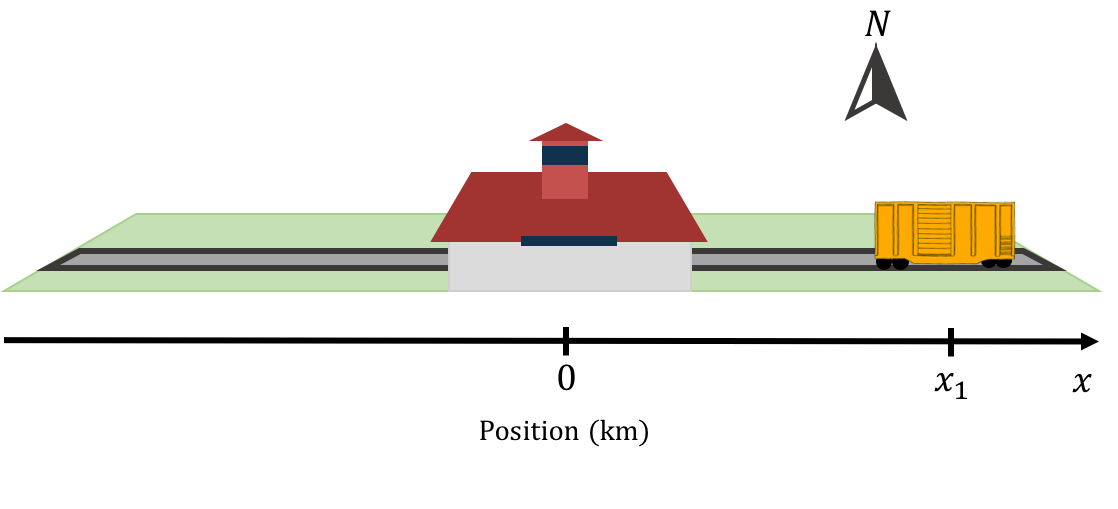
\includegraphics[width=1\linewidth]{files/1daxistrain-89ff23f72498890e6d3c8de8684b986f.png}
\caption[]{A 1d coordinate system describing the position of a train. The Kingston train station is the origin and the East side of the track corresponds to positive values of $x$. The train is located at position $x_1$.}
\label{fig:Vectors:1daxistrain}
\end{figure}

\paragraph{2D Coordinate systems}

\begin{figure}[!htbp]
\centering
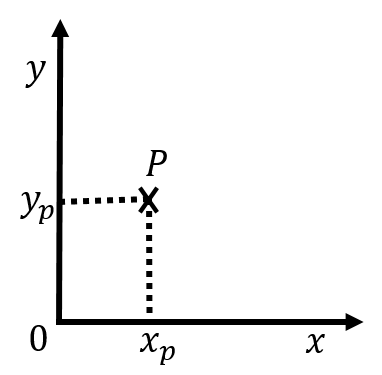
\includegraphics[width=0.375\linewidth]{files/xyp-2af1b012bf7e8142d72db01102577ea1.png}
\caption[]{Example of Cartesian coordinate system and a point $P$ with coordinates $(x_p,y_p)$.}
\label{fig:Vectors:xyp}
\end{figure}

To describe the position of an object in two dimensions (e.g. a marble rolling on a table), we need to specify two numbers. The easiest way to do this is to define two axes, $x$ and $y$, whose origin and direction we must define. Figure~\ref{fig:Vectors:xyp} shows an example of such a coordinate system. Although it is not necessary to do so, we chose $x$ and $y$ axes that are perpendicular to each other. The origin of the coordinate system is where the two axes intersect. One is free to choose any two directions for the axes (as long as they are not parallel). However, choosing axes that are perpendicular (a ``Cartesian'' coordinate system) is usually the most convenient.

To fully describe the position of an object, we must specify both its position along the $x$ and $y$ axes. For example, point $P$ in Figure~\ref{fig:Vectors:xyp} has two \textbf{coordinates}, $x_p$ and $y_p$, that define its position. The $x$ coordinate is found by drawing a line through $P$ that is parallel to the $y$ axis and is given by the intersection of that line with the $x$ axis. The $y$ coordinate is found by drawing a line through point $P$ that is parallel to the $x$ axis and is given by the intersection of that line with the $y$ axis.

\begin{framed}
\textbf{Checkpoint 3.1}\\
Figure~\ref{fig:Vectors:xyslant} shows a coordinate system that is not orthogonal (where the $x$ and $y$ axes are not perpendicular). Which value on the figure correctly indicates the $y$ coordinate of point $P$?

\begin{figure}[!htbp]
\centering
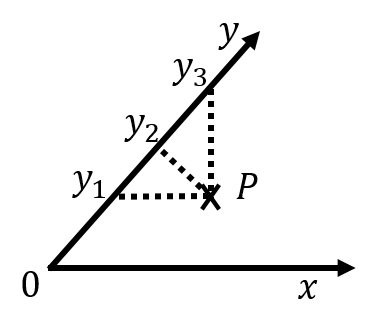
\includegraphics[width=0.375\linewidth]{files/xyslant-b599cfc4e7acffafabef336001b883bd.png}
\caption[]{A non-orthogonal coordinate system (the $x$ and $y$ axes are not perpendicular).}
\label{fig:Vectors:xyslant}
\end{figure}

\begin{enumerate}
\item $y_1$
\item $y_2$
\item $y_3$
\end{enumerate}

\begin{framed}
\textbf{Answer}\\
\begin{enumerate}
\item
\end{enumerate}
\end{framed}
\end{framed}

The most common choice of coordinate system in two dimensions is the Cartesian coordinate system that we just described, where the $x$ and $y$ axes are perpendicular and share a common origin, as shown in Figure~\ref{fig:Vectors:xyp}. When applicable, by convention, we usually choose the $y$ axis to correspond to the vertical direction.

Another common choice is a ``polar'' coordinate system, where the position of an object is specified by a distance to the origin, $r$, and an angle, $\theta$, relative to a specified direction, as shown in Figure~\ref{fig:Vectors:polarp}. Often, a polar coordinate system is defined alongside a Cartesian system, so that $r$ is the distance to the origin of the Cartesian system and $\theta$ is the angle with respect to the $x$ axis.

\begin{figure}[!htbp]
\centering
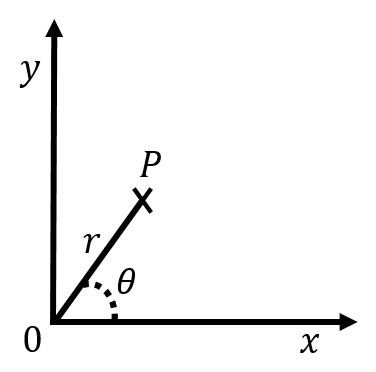
\includegraphics[width=0.375\linewidth]{files/polarp-b3609563a44566297bf1560f08c6e582.png}
\caption[]{Example of a polar coordinate system and a point $P$ with coordinates $(r,\theta)$.}
\label{fig:Vectors:polarp }
\end{figure}

One can easily convert between the two Cartesian coordinates, $x$ and $y$, and the two corresponding polar coordinates, $r$ and $\theta$:
\begin{align*}
x&=r\cos(\theta)\\
y&=r\sin(\theta)\\
r&=\sqrt{x^2+y^2}\\
\tan(\theta) &= \frac{y}{x}
\end{align*}
Polar coordinates are often used to describe the motion of an object moving around a circle, as this means that only one of the coordinates ($\theta$) changes with time (if the origin of the coordinate system is chosen to coincide with the centre of the circle).

\paragraph{3D Coordinate systems}

In three dimensions, we need to specify three numbers to describe the position of an object (e.g. a bird flying in the air). In a three dimensional Cartesian coordinate system, we simply add a third axis, $z$, that is mutually perpendicular to both $x$ and $y$. The position of an object can then be specified by using the three coordinates, $x$, $y$, and $z$. By convention, we use the $z$ axis to be the vertical direction in three dimensions.

Two additional coordinate systems are common in three dimensions: ``cylindrical'' and ``spherical'' coordinates. All three systems are illustrated in Figure~\ref{fig:Vectors:3dcoords} superimposed onto the Cartesian system.

\begin{figure}[!htbp]
\centering
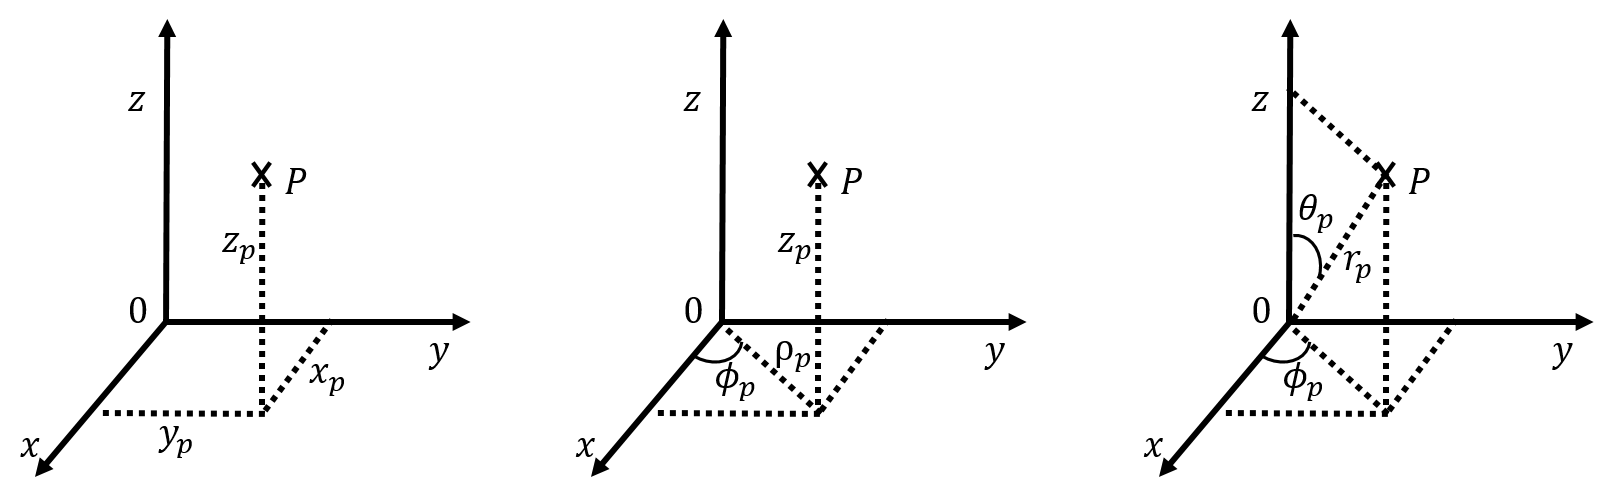
\includegraphics[width=1\linewidth]{files/3dcoords-a3f8711ee5b02abddd6686166e147e2c.png}
\caption[]{Cartesian (left), cylindrical (centre) and spherical (right) coordinate systems used in three dimensions. The $y$ and $z$ axes are in the plane of the page, whereas the $x$ axis comes out of the page.}
\label{fig:Vectors:3dcoords}
\end{figure}

Cylindrical coordinates can be thought of as an extension of the polar coordinates. We keep the same Cartesian coordinate $z$ to indicate the height above the $xy$ plane, however, we use the \textit{azimuthal angle}, $\phi$, and the radius, $\rho$, to describe the position of the projection of a point onto the $xy$ plane. $\phi$ is the angle between the $x$ axis and the line from the origin to the projection of the point in the $xy$ plane and $\rho$ is the distance between the point and the $z$ axis. Thus, cylindrical coordinates are very similar to the polar coordinate system introduced in two dimensions, except with the addition of the $z$ coordinate. Cylindrical coordinates are useful for describing situations with azimuthal symmetry, such as the motion along the surface of a cylinder. For example, consider point $P$ in Figure~\ref{fig:Vectors:cylindricalcoordinates}. Point $P$ is located a distance $\rho$ from the $z$ axis, as it is located on the surface of the cylinder (the circular end of the cylinder has a radius $\rho$). Point $P$ is a height $z$ above the $xy$ plane, and a line from the $z$ axis to point $P$ makes an angle $\phi$ with the $x$ axis.

\begin{figure}[!htbp]
\centering
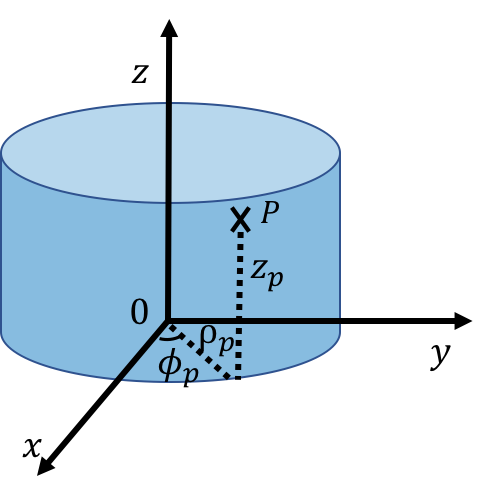
\includegraphics[width=0.375\linewidth]{files/cylindricalcoordinat-e292782c0e16ae0711a2164dbdb614f9.png}
\caption[]{Describing the position of $P$, located on the surface of a cylinder, in cylindrical coordinates.}
\label{fig:Vectors:cylindricalcoordinates}
\end{figure}

The cylindrical coordinates are related to the Cartesian coordinates by:
\begin{align*}
\rho &= \sqrt{x^2+y^2}\\
\tan(\phi) &= \frac{y}{x}\\
z&=z
\end{align*}
In spherical coordinates, a point $P$ is described by the radius, $r$, the \textit{polar angle} $\theta$, and the \textit{azimuthal angle}, $\phi$. The radius is the distance between the point and the origin. The polar angle is the angle with the $z$ axis that is made by the line from the origin to the point. The azimuthal angle is defined in the same way as in polar coordinates. Note that the value of $\phi$ must be between 0 and $2\pi$, whereas the value of $\theta$ must be between 0 and $\pi$.

Spherical coordinates are useful for describing situations that have spherical symmetry, such as a person walking on the surface of the Earth, since the radial coordinate will not change. For example, this is shown with Point $P$ in Figure~\ref{fig:Vectors:sphericalcoordinates}, located on the surface of a sphere of radius $r$.

\begin{figure}[!htbp]
\centering
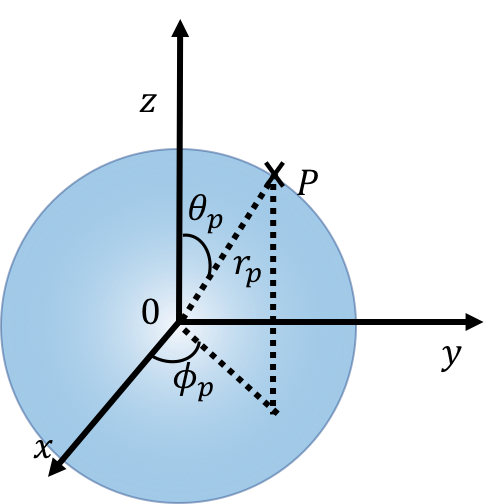
\includegraphics[width=0.375\linewidth]{files/sphericalcoordinates-c774e1b2f767c663403face0501b2dda.png}
\caption[]{Describing the position of $P$, located on the surface of a sphere, in spherical coordinates.}
\label{fig:Vectors:sphericalcoordinates}
\end{figure}

The spherical coordinates are related to the Cartesian coordinates by:
\begin{align*}
r &= \sqrt{x^2+y^2+z^2}\\
\cos(\theta) &= \frac{z}{r}=\frac{z}{\sqrt{x^2+y^2+z^2}}\\
\tan(\phi) &= \frac{y}{x}\\
\end{align*}

\subsubsection{Vectors}

So far, we have seen how to use a coordinate system to describe the position of a single point in space relative to an origin. In this section, we introduce the notion of a ``vector'', which allows us to describe quantities that have a \textbf{magnitude} and a \textbf{direction}. For example, you can use a vector to describe the fact that you walked {\textbackslash}SI\{5\}\{km\} in the North direction. A vector can be visualized by an arrow. The length of the arrow is the magnitude that we wish to describe, and the direction of the arrow corresponds to the direction that we would like to describe.

Unlike a point in space, vectors \textbf{have no location}. That is, vectors are simply an arrow, and you can choose to draw that arrow anywhere you like. In two dimensional space, one requires two numbers to completely define a vector. In three dimensional space, one requires three numbers to completely define a vector. Figure~\ref{fig:Vectors:dvec} shows a two dimensional vector, $\vec d$, twice. Because both arrows in the figure have the same magnitude and direction, they represent the \textit{same} vector. When we refer to quantities that are vectors, we usually draw an arrow on top of the quantity ($\vec d$) to indicate that they are vectors. We use the word ``scalar'' to refer to numbers that are not vectors (a regular number is thus also called a scalar to distinguish it from a quantity that is a vector).

\begin{figure}[!htbp]
\centering
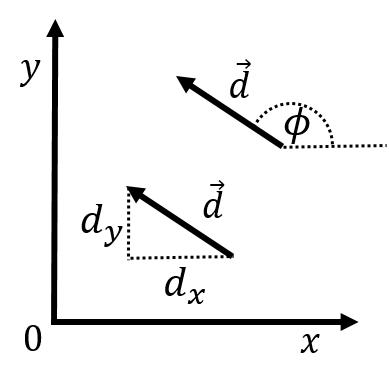
\includegraphics[width=0.375\linewidth]{files/dvec-3a378ef1835699572191f35e5e90f3f5.png}
\caption[]{A vector $\vec d$ shown twice, once with its Cartesian components ($d_x$, $d_y$) and once with its magnitude and direction ($d$, $\phi$).}
\label{fig:Vectors:dvec}
\end{figure}

In analogy with coordinate systems, we have multiple ways to choose the numbers that we use to describe the vector. The most convenient choice is usually to use the ``Cartesian components'' of the vector which correspond to the length of the vector when projected onto a Cartesian coordinate system. For example, in Figure~\ref{fig:Vectors:dvec}, the Cartesian components of the vector $\vec d$ are labelled as ($d_x$, $d_y$) indicating that the vector has a length of $d_x$ in the $x$ direction and $d_y$ in the $y$ direction. Furthermore, the number $d_x$ is negative, since the vector points in the negative $x$ direction. Another common choice is to use the length of the vector, which we label $d$ (the name of the vector without the arrow on top), and the angle, $\phi$ that the vector makes with the $x$-axis, as illustrated in Figure~\ref{fig:Vectors:dvec}. In terms of the two dimensional Cartesian components, the magnitude of the vector is given by:
\begin{align*}
d&= ||\vec d||= \sqrt{d_x^2+d_y^2}
\end{align*}
where we also introduced the notation that placing two vertical bars around a vector ($||\vec d||$) is used to indicated its magnitude. Note that in three dimensions, it is usually not convenient to specify the direction unless the vector lies in one of the planes defined by the coordinate system (e.g the $xy$ plane). In three dimensions, it is usually most convenient to specify the three Cartesian components.

\paragraph{Unit vectors}

A special category of vectors is ``unit vectors'', which are simply vectors that have a length (magnitude) of 1 (in whichever units the coordinate system is defined). Unit vectors are particularly useful for indicating direction. For example, in Figure~\ref{fig:Vectors:dvec}, we may be interested in indicating the direction of the vector $\vec d$. Unit vectors are denoted by using a ``hat'' instead of an arrow. Thus, the vector $\hat d$, is the vector of length 1 that points in the same direction as $\vec d$. The (Cartesian) components of $\hat d$ are easily found by dividing the corresponding components of $\vec d$ by $d$ (the magnitude):
\begin{align*}
(\hat d)_x &= \frac{d_x}{d}=\frac{d_x}{\sqrt{d_x^2+d_y^2}}\\
(\hat d)_y &= \frac{d_y}{d}=\frac{d_y}{\sqrt{d_x^2+d_y^2}}\\
\therefore d &= ||\hat d||=\sqrt{(\hat d)_x^2+(\hat d)_y^2}=\sqrt{\frac{d_x^2}{d_x^2+d_y^2}+\frac{d_y^2}{d_x^2+d_y^2}}=1
\end{align*}

A specific type of unit vector is the units vectors that are parallel to the axes of the coordinate system. Those vectors are denoted $\hat x$, $\hat y$, $\hat z$ (and sometimes $\hat i$, $\hat j$, $\hat k$ or $\hat e_x$, $\hat e_y$, $\hat e_z$) for the $x$, $y$, and $z$ axes, respectively. Thus, the vector $d\hat{x}$, is the vector of length $d$ that points in the positive $x$ direction.

\paragraph{Notations and representation of vectors}

There are multiple notations for describing a vector using its components. The following are all equivalent ways to write down the vector $\vec d$ in terms of its components $d_x$ and $d_y$:
\begin{align*}
\vec d &= (d_x,d_y)\quad&\text{row vector}\\
       &=\begin{pmatrix}
           d_x \\
           d_y \\
         \end{pmatrix}\quad&\text{column vector}\\
         &= d_x\hat x +d_y \hat y\quad&\text{using }\hat x,\;\hat y\\
         &=d_x\hat i +d_y \hat j \quad&\text{using }\hat i,\;\hat j
\end{align*}
The vectors $\hat x$ ($\hat i$) and $\hat y$ ($\hat j$) are unit vectors in $x$ and $y$ directions respectively.
For example, the unit vector $\hat y$ can be written down as (0,1) in two dimensions or (0,1,0) in three dimensions, using the row notation.

\begin{framed}
\textbf{Checkpoint 3.2}\\
What is the magnitude (the length) of the vector $5\hat x -2\hat y$?

\begin{enumerate}
\item 3.0
\item 5.4
\item 7.0
\item 10.0
\end{enumerate}

\begin{framed}
\textbf{Answer}\\
\begin{enumerate}[resume]
\item
\end{enumerate}
\end{framed}
\end{framed}

Illustrating a vector graphically in two dimensions is straightforward, but difficult in three dimensions. To help remedy this, a notation is introduced in order to draw vectors that point in or out of the page (perpendicular to the plane of the page). The notation comes from imagining that the vector is an archery arrow. If the vector is coming out of the page (at you!), then you would see the head of the arrow, which we represent as a circle with a dot (the dot is the point of the arrow, the circle is the base of the conically shaped arrowhead). If instead, the vector points into the page, then you would see the back of the arrow, which we represent as a cross (the cross being the feathers in the tail of the arrow). This is illustrated in Figure~\ref{fig:Vectors:vector3d}.

\begin{figure}[!htbp]
\centering
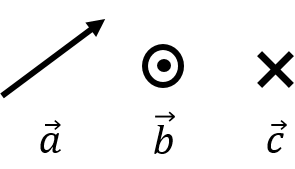
\includegraphics[width=0.375\linewidth]{files/vector3d-3bea86fda2d25a5ff5ca79d247637439.png}
\caption[]{Geometric representation of three vectors. The vector $\vec a$ lies in the plane of the page, the vector $\vec b$ is pointing out of the page, and the vector $\vec c$ is pointing into the page.}
\label{fig:Vectors:vector3d}
\end{figure}

\subsubsection{Vector algebra}

In this section, we describe the various algebraic operations that can be performed using vectors.

\paragraph{Multiplication/division of a vector by a scalar}

One can multiply (or divide) a vector by a scalar (a number). Suppose that we are given a vector $\vec v=(v_x, v_y, v_z)$ and a scalar $a$. The multiplication $a\vec v$ is defined to be a new vector, say $\vec w$, whose components are the components of $\vec v$ multiplied by $a$:
\begin{align*}
\vec w = a\vec v = (av_x, a v_y, av_z)
\end{align*}
Similarly, the division of a vector by a scalar is defined analogously by dividing each Cartesian component by the scalar::
\begin{align*}
\vec w = \frac{\vec v}{a} = \left(\frac{v_x}{a}, \frac{v_y}{a}, \frac{v_z}{a}\right)
\end{align*}
\begin{framed}
\textbf{Checkpoint 3.3}\\
What happens to the length of a vector if the vector is multiplied by 2 (a scalar)?

\begin{enumerate}
\item The length doubles
\item The length is halved
\item The length is quadrupled
\item It depends on the direction of the vector
\end{enumerate}

\begin{framed}
\textbf{Answer}\\
\begin{enumerate}
\item
\end{enumerate}
\end{framed}
\end{framed}

In particular, this makes it easy to determine the unit vector, $\hat v$, that points in the same direction as $\vec v$:
\begin{align*}
\hat v = \frac{\vec v}{v}
\end{align*}
where $v$ is the (scalar) magnitude of $\vec v$.

\paragraph{Addition/subtraction of two vectors}

The sum of two vectors, $\vec a$ and $\vec b$, is found by adding the components of the two vectors. Similarly, the difference between two vectors is found by subtracting the components. For example, if $\vec c=\vec a+\vec b$, the components of $\vec c$ are given by:
\begin{align*}
\vec c &= \vec a + \vec b = \begin{pmatrix}
           a_x \\
           a_y \\
         \end{pmatrix} + \begin{pmatrix}
           b_x \\
           b_y \\
         \end{pmatrix}\\
        \therefore \begin{pmatrix}
           c_x \\
           c_y \\
         \end{pmatrix} &=\begin{pmatrix}
           a_x+b_x \\
           a_y+b_y \\
         \end{pmatrix}
\end{align*}
where we chose to use the ``column vector'' notation. The column vector notation highlights the fact that the algebra (addition, subtraction) is performed independently on the $x$ and $y$ components. We can thus write this sum equivalently as two scalar equations, one for each coordinate:
\begin{align*}
c_x &= a_x+b_x\\
c_y &= a_y+b_y
\end{align*}
Vectors can thus be used as a short-hand notation for representing multiple equations (one equation per component). When we use vectors to write an equation such as:
\begin{align*}
\vec F = m\vec a
\end{align*}
we really mean that there is one scalar equation per component of the vectors:
\begin{align*}
F_x &= ma_x\\
F_y &= ma_y\\
F_z &= ma_z
\end{align*}

\begin{framed}
\textbf{Example 3.1}\\
Given two vectors, $\vec a=2\hat x+3\hat y$, and $\vec b=5\hat x -2\hat y$, calculate the vector $\vec c= 2\vec a - 3\vec b$.

\begin{framed}
\textbf{Solution}\\
This can easily be solved algebraically by collecting terms for each component, $\hat x$ and $\hat y$:
\begin{align*}
\vec c &= 2\vec a- 3\vec b\\
&=2 (2\hat x+3\hat y) - 3 (5\hat x-2\hat y) \\
&=(4\hat x+6\hat y)-(15\hat x-6\hat y) \\
&=(4-15)\hat x + (6+6) \hat y\\
&= -11 \hat x + 12 \hat y
\end{align*}
We can think of these operations as being performed independently on the components:
\begin{align*}
c_x&=2a_x-3b_x=-11\\
c_y&=2a_y-3b_y=12
\end{align*}
\end{framed}
\end{framed}

Geometrically, one can easily visualize the addition and subtraction of vectors. This is illustrated in Figure~\ref{fig:Vectors:aplusbvec} for the case of adding vectors $\vec a$ and $\vec b$ to get the vector $\vec c$. Geometrically, the sum of the vectors $\vec a$ and $\vec b$ (sometimes also called the ``resultant'') can be found by:

\begin{enumerate}
\item Placing the ``tail'' of vector $\vec b$ at the ``head'' of $\vec a$ (think of an arrow, the pointy part is the head and the feathery part is the tail)
\item Drawing the vector that goes from the tail of vector $\vec a$ to the head of vector $\vec b$.
\end{enumerate}

\begin{figure}[!htbp]
\centering
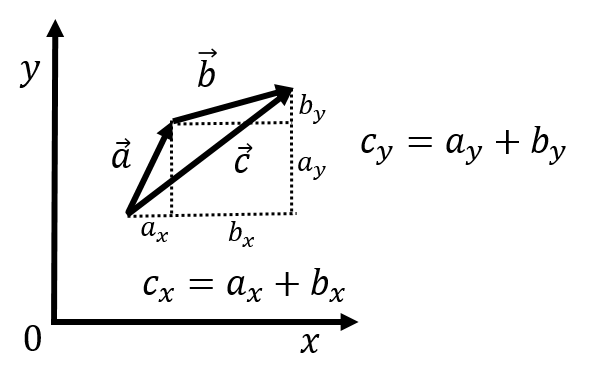
\includegraphics[width=0.625\linewidth]{files/aplusbvec-61cf3b3366ea729ed569bbf242b101f4.png}
\caption[]{Geometric addition of the vectors $\vec a$ and $\vec b$ by placing them ``head to tail''.}
\label{fig:Vectors:aplusbvec}
\end{figure}

Subtracting two vectors geometrically is done in the same way as addition. For example, the vector $\vec c$, given by $\vec c=\vec a -\vec b$ can also be expressed as $\vec c = \vec a + ( -1) \vec b$. That is, first multiply the vector $\vec b$ by minus 1 (which just reverses its direction), then add that vector, ``head to tail'', to the vector $\vec a$.

Now that we know how to add vectors, we can better understand the notation $\vec a = a_x \hat x+ a_y\hat y$. This is not simply a notation, but is in fact algebraically correct. It means: ``multiply the vector $\hat x$ by $a_x$ (thus giving it a length of $a_x$) and then add $a_y$ times the vector $\hat y$''. This is illustrated in Figure~\ref{fig:Vectors:acomponents}, which shows the unit vectors, $\hat x$ and $\hat y$, which are then multiplied by $a_x$ and $a_y$, respectively, and then added together ``head to tail''.

\begin{figure}[!htbp]
\centering
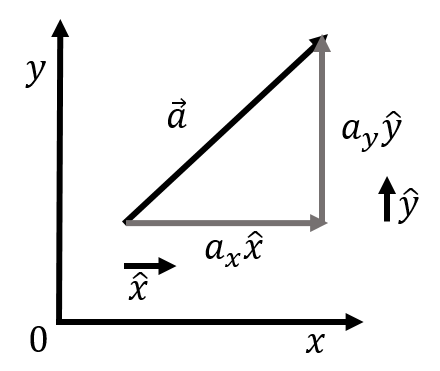
\includegraphics[width=0.375\linewidth]{files/acomponents-4093cabc11330a40aa3366764b387b46.png}
\caption[]{Illustration that the notation $\vec a = a_x \hat x+ a_y\hat y$ is in fact the vector addition of $a_x \hat x$ and $a_y \hat y$.}
\label{fig:Vectors:acomponents}
\end{figure}

\paragraph{The scalar product}\label{sec:Vectors:scalarproduct}

There are two ways to ``multiply'' vectors: the ``scalar product'' and the ``vector product''. The scalar product (or ``dot product'') takes two vectors and results in a scalar (a number). The vector product (or ``cross product'') takes two vectors and results in a third vector.

The scalar product, $\vec a \cdot \vec b$, of two vectors $\vec a$ and $\vec b$, is defined as the following:
\begin{align*}
\vec a \cdot \vec b=a_xb_x +a_yb_y
\end{align*}
That is, one multiplies the individual components of the two vectors and then adds those products for each component. This is easily extended to the three dimensional case by adding a term $a_zb_z$ to the sum. The scalar product is also related to the angle between the two vectors when the vectors are placed ``tail to tail'', as in Figure~\ref{fig:Vectors:scalarproduct}
\begin{align*}
\vec a \cdot \vec b= ab\cos\theta
\end{align*}

\begin{figure}[!htbp]
\centering
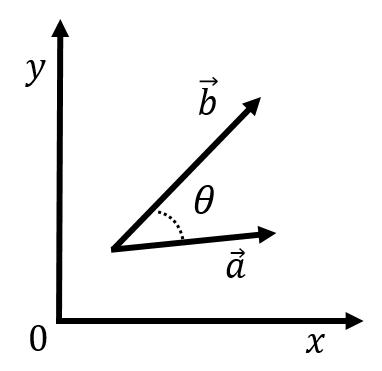
\includegraphics[width=0.375\linewidth]{files/scalarproduct-76eac9ae093e2d1f0c79b032fc805048.png}
\caption[]{Illustration of the angle between vectors $\vec a$ and $\vec b$ when these are placed tail to tail.}
\label{fig:Vectors:scalarproduct}
\end{figure}

The scalar product between two vectors of a fixed length will be maximal when the two vectors are parallel ($\cos\theta=1$) and zero when the vectors are perpendicular ($\cos\theta =0$). The scalar product is thus useful when we want to calculate quantities that are maximal when two vectors are parallel.

\begin{framed}
\textbf{Checkpoint 3.4}\\
The vectors $\vec a$ and $\vec b$ in the three diagrams below have the same magnitude. Order the diagrams from the one that gives the smallest scalar product $\vec a\cdot \vec b$ to the largest scalar product.

\begin{figure}[!htbp]
\centering
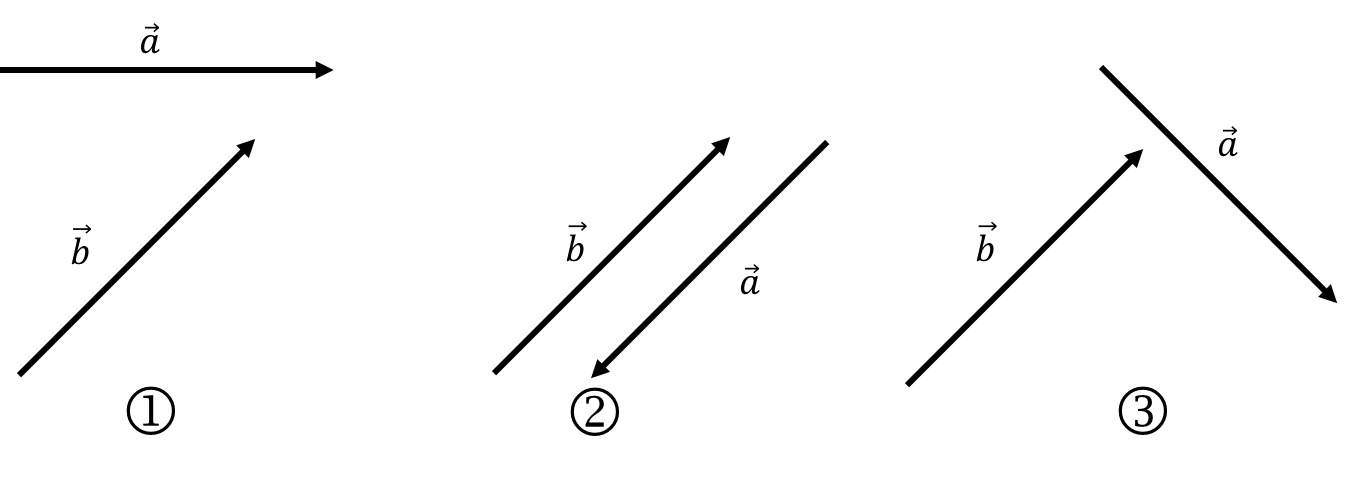
\includegraphics[width=1\linewidth]{files/vectororder-853fd2d5b8f2fb40756bb18b5b6128a5.png}
\caption[]{Put these in order of the magnitude of their scalar product.}
\label{fig:Vectors:scalarproductorder}
\end{figure}

\begin{framed}
\textbf{Answer}\\
$3<1<2$
\end{framed}
\end{framed}

\paragraph{The vector product}\label{sec:Vectors:vectorproduct}

The vector (or cross) product takes two vectors to produce a third vector that is \textbf{mutually perpendicular} to both vectors. The vector product only has meaning in three dimensions. Two vectors that are not co-linear, meaning they can not be arranged so that they lie along the same line, can always be used to define a plane in three dimensions. The cross product of those two vectors will give a third vector that is perpendicular to the plane (making it perpendicular to both vectors).

Algebraically, the three components of the vector product, $\vec a\times \vec b$, of vectors $\vec a$ and $\vec b$ are found as follows:
\begin{equation}
\label{eqn:Vectors:crossproduct}
\vec a \times \vec b =\begin{pmatrix}
           a_yb_z - a_z b_y\\
           a_zb_x - a_x b_z\\
           a_xb_y - a_y b_x\\
         \end{pmatrix}
\end{equation}

One important property to note is that $\vec a \times \vec b = -\vec b \times \vec a$; that is, the cross product is not commutative (the order matters). The magnitude of the vector obtained by a cross product is given by:
\begin{equation}
\label{eqn:Vectors:crossproductmag}
||\vec a \times \vec b ||=ab\sin\theta
\end{equation}
where $\theta$ is the angle between the vectors $\vec a$ and $\vec b$ when these are placed tail to tail (Figure~\ref{fig:Vectors:scalarproduct}). The vector resulting from a cross product will be null (have a zero length) if the vectors $\vec a$ and $\vec b$ are parallel, and will have a maximal length when these are perpendicular. The cross product is useful to determine quantities that are maximal when two vectors are perpendicular.

Geometrically, one can determine the direction of the cross product of two vectors by using a ``right hand rule''. To distinguish it from another right hand rule (see Section~\ref{sec:Vectors:rotationalmotion}), we will call it ``the right hand rule for the cross product''). This is done by using your right hand, aligning your thumb with the first vector and your index with the second vector. The cross product will point in the direction of your middle finger (when you hold your middle finger perpendicular to the other two fingers). This is illustrated in Figure~\ref{fig:Vectors:righthandrule}. Thus, you can often avoid using equation (\ref{eqn:Vectors:crossproduct}) and instead use the right hand rule to determine the direction of the cross product and equation (\ref{eqn:Vectors:crossproductmag}) to find its magnitude.

\begin{figure}[!htbp]
\centering
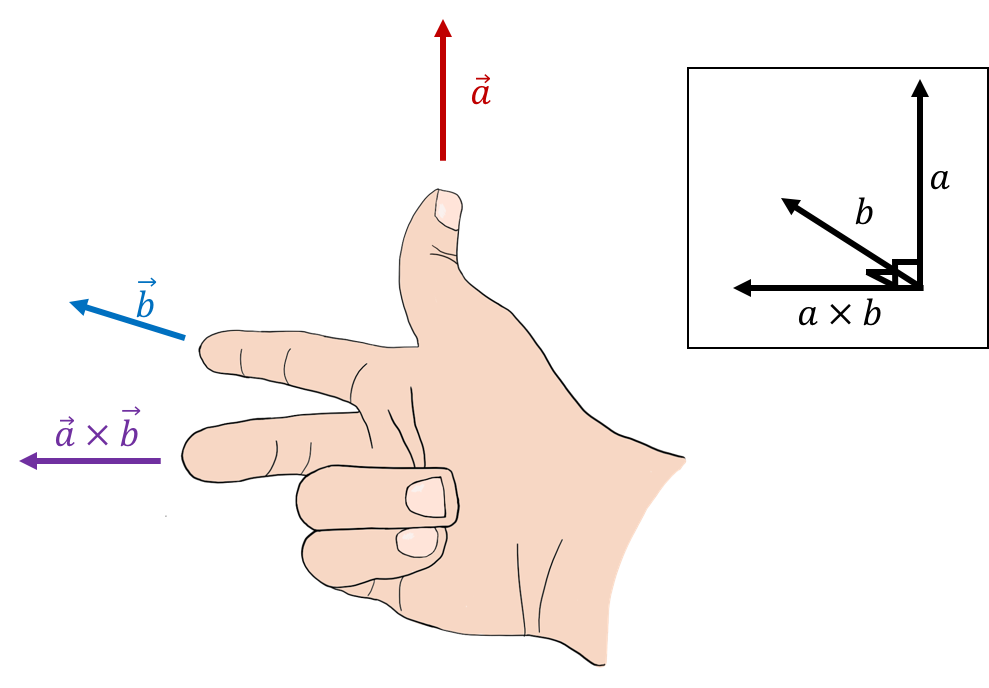
\includegraphics[width=1\linewidth]{files/righthandrule-8ae8bedd142f4f76e321e2f318eae4aa.png}
\caption[]{Using the right hand rule for cross products to find the direction of the cross product of vectors $\vec a$ (upwards) and $\vec b$ (into the page).}
\label{fig:Vectors:righthandrule }
\end{figure}

The unit vectors that define a coordinate system have the following properties relative to the cross product:
\begin{align*}
\hat x \times \hat y &= \hat z\\
\hat y \times \hat z &= \hat x\\
\hat z \times \hat x &= \hat y\\
\end{align*}
For these properties to be correct, it should be noted that the direction of the $z$ axis in three dimensions is specified by the choice of $x$ and $y$ axes. That is, one can freely choose the direction of the $x$ and $y$ axes, which then define a plane to which the $z$ axis will be perpendicular. The direction of the $z$ axis must be chosen so that $\hat x \times \hat y = \hat z$ (this guarantees that the coordinate system is ``right handed''), as in Figure~\ref{fig:Vectors:xyzaxis}.

\begin{figure}[!htbp]
\centering
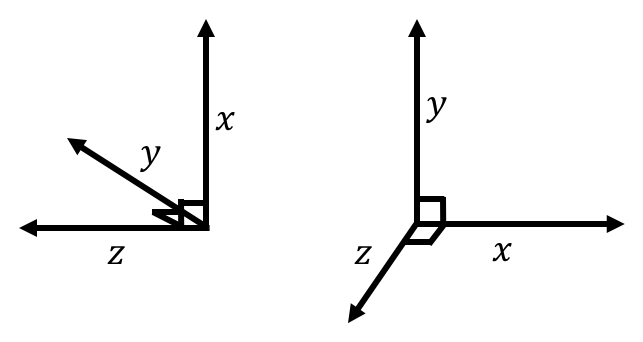
\includegraphics[width=0.625\linewidth]{files/xyzaxis-9e9577552478578827b53fb21afae42b.png}
\caption[]{Two possible orientations for a three dimensional coordinate system. You can confirm using the right hand rule that the $z$ axis is the cross product $\hat x \times \hat y$.}
\label{fig:Vectors:xyzaxis}
\end{figure}

\subsubsection{Example uses of vectors in physics}

This section gives a quick overview of some applications of vectors in physics.

\paragraph{Kinematics and vector equations}

Kinematics is the description of the position and motion of an object (Chapters \href{\#chapter:describingmotionin1d}{} and \href{\#chapter:describingmotioninnd}{}). The laws of physics are the principles that ultimately allow us to determine how the position of an object changes with time. For example, Newton's Laws are a mathematical framework that introduce the concepts of force and mass in order to model and determine how an object will move through space.

We often use a \textbf{position vector}, $\vec r(t)$, to describe the position of an object as a function of time. Because the object can move, the position vector is a function of time. A position vector is a special vector in the sense that it should be considered to be fixed in space; the position vector for an object points from the origin of a coordinate system to the location of the object.

The three components of the position vector in Cartesian coordinates, are the $x$, $y$, and $z$ coordinates of the object:
\begin{align*}
\vec r(t) = \begin{pmatrix}
           x(t) \\
           y(t) \\
           z(t) \\
         \end{pmatrix}
\end{align*}
where the three coordinates of the object are functions of time if the object can move. Suppose that the object was initially at position $\vec r_1=(x_1, y_1, z_1)$ at some time $t=t_1$, and that later, at time $t=t_2$, the object was at as second position, $\vec r_2=(x_2, y_2, z_2)$. We can define the \textbf{displacement vector}, $\vec  d$, as the vector from position $\vec r_1$ to position $\vec r_2$:
\begin{align*}
 \vec d = \vec r_2 - \vec r_1 =\begin{pmatrix}
           x_2-x_1 \\
           y_2-y_1 \\
           z_2-z_1 \\
         \end{pmatrix} = \begin{pmatrix}
           \Delta x \\
           \Delta y \\
           \Delta z \\
         \end{pmatrix}
\end{align*}
The displacement vector is such that one can add the vector $\vec d$ to the vector $\vec r_1$ to describe the new position of the object at time $t_2$:
\begin{align*}
\vec d &= \vec r_2 - \vec r_1\\
\therefore \vec r_2 &= \vec r_1 + \vec d
\end{align*}
The components of the displacement vector, $\Delta x$, $\Delta y$, and $\Delta z$ correspond to the displacements (the distance travelled) along the $x$, $y$, and $z$ axes, respectively. This is illustrated for the two dimensional case in Figure~\ref{fig:Vectors:xydvec}.

\begin{figure}[!htbp]
\centering
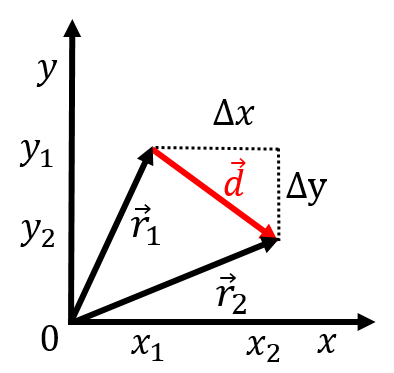
\includegraphics[width=0.375\linewidth]{files/xydvec-47b3c4d0a25582caecba219c976e060e.png}
\caption[]{Illustration of a displacement vector, $\vec d = \vec r_2 -\vec r_1$, for an object that was located at position $\vec r_1$ at time $t_1$ and at position $\vec r_2$ at time $t_2$.}
\label{fig:Vectors:xydvec}
\end{figure}

The velocity vector of the object, $\vec v=(v_x, v_y, v_z)$, is defined to be the displacement vector, $\vec d$, divided by the amount of time (a scalar) that elapsed, $\Delta t=t_2 -t_1$, while the object moved by the corresponding displacement:
\begin{align*}
\vec v = \frac{\vec d}{\Delta t}=\begin{pmatrix}
           \frac{\Delta x}{\Delta t} \\
           \frac{\Delta y}{\Delta t} \\
           \frac{\Delta z}{\Delta t} \\
         \end{pmatrix}
\end{align*}
We used the property that dividing a vector by a scalar ($\Delta t$) is defined as dividing each component by the scalar. If we write the components of the velocity vector out explicitly, we have:
\begin{align*}
\begin{pmatrix}
           v_x \\
           v_y \\
           v_z \\
         \end{pmatrix} = \begin{pmatrix}
           \frac{\Delta x}{\Delta t} \\
           \frac{\Delta y}{\Delta t} \\
           \frac{\Delta z}{\Delta t}
         \end{pmatrix}
\end{align*}
That is, we can think of each row in this ``vector equation'' as an independent equation. That is, when we write the vector equation:
\begin{align*}
\vec v = \frac{\vec d}{\Delta t}
\end{align*}
we are really just using a shorthand notation for writing the three \textbf{independent} equations that are true for each individual component of the vectors:
\begin{align*}
v_x &= \frac{\Delta x}{\Delta t} \\
v_y &= \frac{\Delta y}{\Delta t} \\
v_z &= \frac{\Delta z}{\Delta t} \\
\end{align*}
Whenever we write an equation using vectors, we are really writing out multiple equations all at once, one for each component. Newton's Second Law:
\begin{align*}
\vec F = m \vec a
\end{align*}
thus corresponds to the three (scalar) equations:
\begin{align*}
F_x &= ma_x\\
F_y &= ma_y\\
F_z &= ma_z\\
\end{align*}

\paragraph{Work and scalar products}

As we will see, ``work'' is a scalar quantity that allows us to determine the change in the speed (squared) of an object that results from a force exerted over a particular displacement (Chapter Section~\ref{chap:workenergy}). Both force and the displacement are vector quantities (a force has a magnitude and is exerted in a particular direction). The work, $W$, done by a force, $\vec F$, over a displacements, $\vec d$, is defined as:
\begin{align*}
W = \vec F \cdot \vec d
\end{align*}
The work energy theorem tells us that this work is related to the change in speed squared of the object as it moves along the displacement vector $d$. If the work is zero, the object has the same speed at the beginning and end of the displacement. If the work is positive, the object is moving faster at the end of the displacement (and slower if the work is negative). A one dimensional example is shown in Figure~\ref{fig:Vectors:work_scalarprod}, which shows a force $\vec F$ being applied to a block as it slides along the ground over a distance $d$ (represented by the displacement vector $\vec d$).

\begin{figure}[!htbp]
\centering
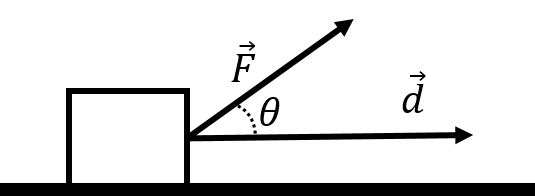
\includegraphics[width=0.625\linewidth]{files/work_scalarprod-31c94373518d315f6fb766143522e2b4.png}
\caption[]{Example of a force $\vec F$ being applied on an object as it moves along the displacement vector $\vec d$.}
\label{fig:Vectors:work_scalarprod}
\end{figure}

Intuitively, it makes sense that only the horizontal component of the force would contribute to changing the speed of the object as it moves along the horizontal trajectory defined by the vector $\vec d$. The vertical component of the force does not contribute to changing the speed of the object. Thus, the work (the change in speed), should only depend on the component of the force that is parallel to the displacement vector. The scalar product allows us to formalize this in an equation. The scalar product is given by:
\begin{align*}
\vec F \cdot \vec d = Fd\cos\theta = F_{\parallel}d
\end{align*}
where we introduced $F_{\parallel} = F\cos\theta$ as the component of $\vec F$ that is parallel to $\vec d$ (see Figure~\ref{fig:Vectors:work_scalarprod}). The scalar product thus ``picks out'' the component of $\vec F$ that is parallel to $\vec d$, which is exactly what we need to in order for work to make sense.

\paragraph{Using vectors to describe rotational motion}\label{sec:Vectors:rotationalmotion}

Often, we need to describe rotational motion in physics. If an object is rotating, one must specify:

\begin{enumerate}
\item The axis about which the object is rotating
\item The direction about that axis in which the object is rotating (e.g. clockwise or counter-clockwise)
\item How fast the object is rotating
We introduce a new type of vector, an ``axial vector'', to describe this kind of rotational motion. We choose the direction of the vector to be co-linear with the axis of rotation and the magnitude of the vector to represent the speed with which the object is rotating. We are thus left with two choices for the direction of the vector. For example, consider the wheels on a car that is moving away from you (Figure~\ref{fig:vectors:carwheelrotation}, the car is moving into the page).  The axis of rotation is the axis of the wheel, so we know that the vector describing the wheel's rotation (the angular velocity vector) must point either to the left or to the right.
\end{enumerate}

\begin{figure}[!htbp]
\centering
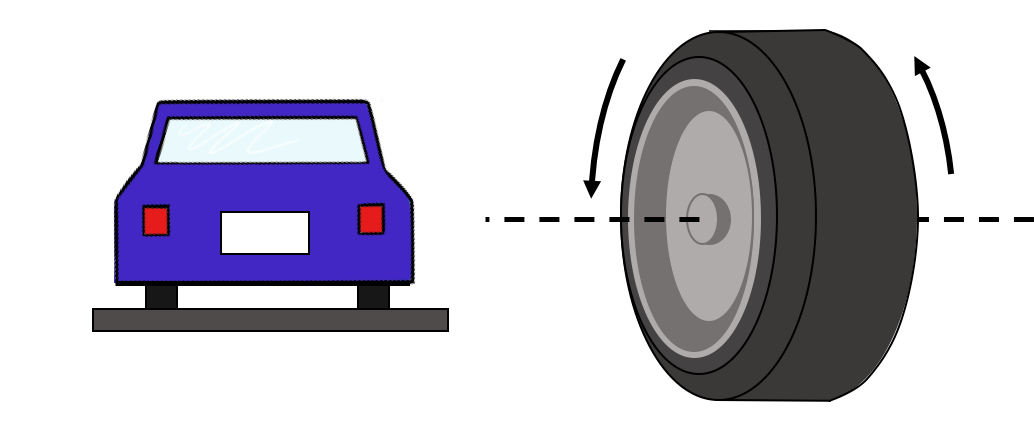
\includegraphics[width=0.625\linewidth]{files/carwheelrotation-c64ab18f43acb3147151239fe27f737b.png}
\caption[]{The wheels on a car that is driving away from you.}
\label{fig:vectors:carwheelrotation}
\end{figure}

We choose the direction of the vector by using another right hand rule. We will refer to this as ``the right hand rule for axial vectors'' to distinguish it from the right hand rule for the cross product.  When using the right hand rule for axial vectors, the vector points in the direction of your thumb when you curl your fingers in the direction of rotation, as in Figure~\ref{fig:vectors:righthandruleaxial}. For the car moving away from you, the wheels will be turning such that the closest point to you is moving up and the furthest point is moving down. Using the right hand rule, we find that the rotation vector points to the left.

\begin{figure}[!htbp]
\centering
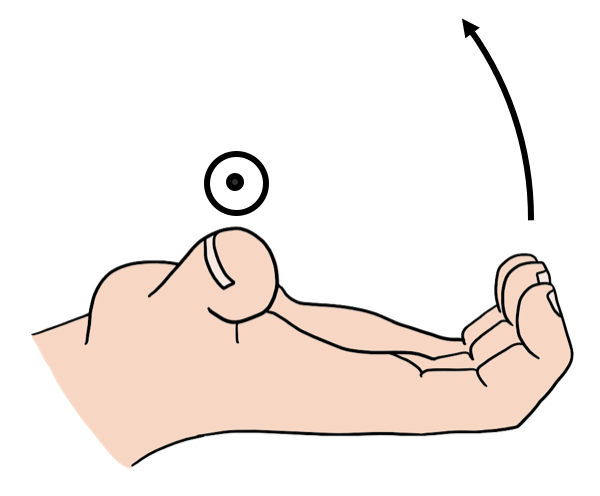
\includegraphics[width=0.375\linewidth]{files/righthandruleaxial-54dbfdc774fe5213371ff87012fb8fd1.png}
\caption[]{Using the right hand rule for axial quantities. In this case, the direction of rotation is counter clockwise when looking at the page (the direction that the fingers curl), so the rotation vector points out of the page (the direction of the thumb).}
\label{fig:vectors:righthandruleaxial}
\end{figure}

We have to distinguish axial vectors from ``true'' vectors because they do not behave like true vectors in all cases.
For instance, imagine that there is a giant mirror that runs parallel to the road (Figure~\ref{fig:vectors:wheelmirror}). When the car is reflected in the mirror, the reflected car will also be moving away from you. This means that the wheels will be turning in the same direction as before, so the rotation vector still points to the left. Now consider a true vector, like a velocity vector. If the velocity vector initially pointed to the left (i.e. if the car was moving to the left), the reflected car would be moving to the \textit{right}. So, we expect a true vector to change directions when it is reflected in this way. Since the rotation vector does not always behave like a true vector, we call it an axial vector or a ``pseudovector.''

\begin{figure}[!htbp]
\centering
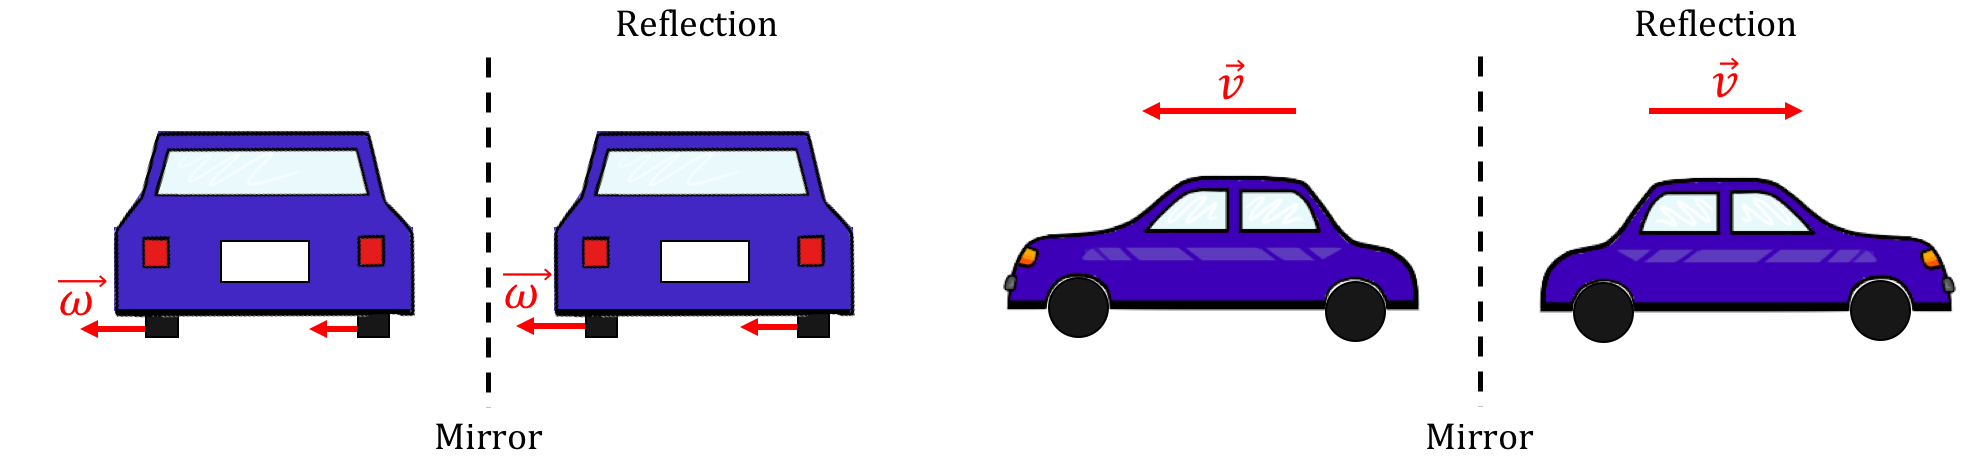
\includegraphics[width=1\linewidth]{files/carwheelmirror-4905ab3ad6241de2b3eb70d85ebdfc48.png}
\caption[]{Left: The angular velocity vector for the rotation of the wheels, $\vec \omega$, which points to the left, also points left in the reflection. Right: The velocity vector, pointing to the left, points to the right in the reflection of the car. The angular velocity vector is called an ``axial'' or ``pseudo'' vector because it does not change direction under a reflection.}
\label{fig:vectors:wheelmirror}
\end{figure}

\paragraph{Torque and vector products}

We will introduce the concept of a torque in order to describe how a force can cause an object to rotate. Consider the disk illustrated in Figure~\ref{fig:Vectors:torque_vectorprod} that is free to rotate about an axis that goes through its centre and that is perpendicular to the plane of the page. A force $\vec F$ is applied at the edge of the disk (imagine pulling on a string attached to the edge of the disk), at a position that is displaced from the axis of rotation by the vector $\vec r$. The torque, $\vec \tau$, of the force about the centre of the disk is defined to be:
\begin{align*}
\vec\tau=\vec r\times \vec F
\end{align*}
and represents how much the force $\vec F$ will contribute to making the disk rotate about its axis. If the force vector were parallel to the vector $\vec r$, the disk would not rotate; if you pull outwards on a disk, it will not rotate about its centre. However, if the force is perpendicular to the vector $\vec r$ (i.e. tangent to the circumference of the disk), then it will maximally cause the disk to rotate. The magnitude of the torque (cross-product) is given by:
\begin{align*}
\tau =rF\sin\theta=F_{\perp}r=Fr_\perp
\end{align*}
where $\theta$ is the angle between the vectors when placed tail to tail, as in the right side of Figure~\ref{fig:Vectors:torque_vectorprod}. In the last two equalities, we have defined $F_\perp=F\sin\theta$ or $r_\perp=r\sin\theta$ to refer to the part of the vector $\vec F$ that is perpendicular to the vector $\vec r$ or the part of the vector $\vec r$ that is perpendicular to the vector $\vec F$. That is, the vector product ``picks out'' the part of a vector that is perpendicular to the other, which is exactly the property that we need for the physical quantity of torque.

\begin{figure}[!htbp]
\centering
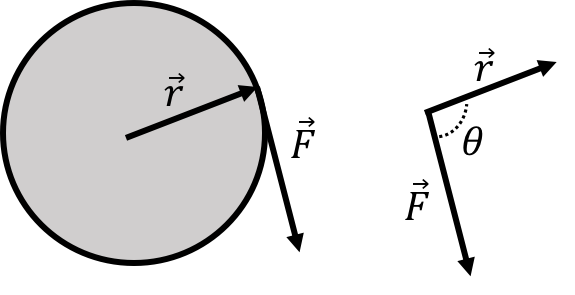
\includegraphics[width=0.7\linewidth]{files/torque_vectorprod-99e945d9629e68374c448a564ccd7e86.png}
\caption[]{A force, $\vec F$, is exerted in the plane of a disk at a position given by the vector $\vec r$ relative to the centre of the disk.}
\label{fig:Vectors:torque_vectorprod}
\end{figure}

\begin{framed}
\textbf{Checkpoint 3.5}\\
Referring to Figure~\ref{fig:Vectors:torque_vectorprod}, in which direction does the torque vector point?

\begin{enumerate}
\item to the right
\item to the left
\item out of the page
\item into the page
\end{enumerate}

\begin{framed}
\textbf{Answer}\\
\begin{enumerate}[resume]
\item
\end{enumerate}
\end{framed}
\end{framed}

\subsubsection{Summary}

Cartesian coordinate systems can be defined using an origin, and mutually perpendicular axes that specify a direction in which each corresponding coordinate increases. The position of a point is described by the coordinates of the point (one coordinate per axis). Polar, cylindrical and spherical coordinate systems can be defined relative to a Cartesian coordinate system and sometimes facilitate the description of situations with cylindrical (azimuthal) or spherical symmetry.

Vectors can be represented by arrows and are quantities that have both a magnitude and a direction, as opposed to ``scalars'', which are simply numbers. Vectors are not fixed in space, so two vectors are equal if they have the same magnitude and direction, regardless of where they are drawn. We place a little arrow above a variable, $\vec d$, to indicate that it is a vector. There are several, equivalent, notations to indicate the components of a vector:
\begin{align*}
\vec d &= (d_x,d_y, d_z)\quad&\text{row vector}\\
       &=\begin{pmatrix}
           d_x \\
           d_y \\
           d_z\\
         \end{pmatrix}\quad&\text{column vector}\\
         &= d_x\hat x +d_y \hat y +d_z \hat z\quad&\text{using }\hat x,\;\hat y,\;\hat z\\
         &=d_x\hat i +d_y \hat j+d_z \hat k \quad&\text{using }\hat i,\;\hat j,\;\hat k
\end{align*}
If we multiply (divide) a vector by a scalar, we multiply (divide) each component of the vector individually by that quantity. As a result, the magnitude of the vector will also be multiplied (divided) by that quantity:
\begin{align*}
a\vec d = \begin{pmatrix}
           ad_x \\
           ad_y \\
           ad_z \\
         \end{pmatrix}
\end{align*}
In particular, we can define a unit vector, $\hat d$, to be a vector of length 1 in the same direction as $\vec d$, by simply dividing $\vec d$ by its magnitude, $d$:
\begin{align*}
\hat d = \frac{\vec d}{d}
\end{align*}
where the magnitude of the vector, $||\vec d|| = d$, expressed in Cartesian coordinates, is given by:
\begin{align*}
||\vec d|| = d =\sqrt{d_x^2+d_y^2+d_z^2}
\end{align*}
We can add two vectors by independently adding the individual components of the vectors:
\begin{align*}
\vec c &= \vec a + \vec b\\
\therefore c_x &= a_x + b_x\\
\therefore c_y &= a_y + b_y\\
\therefore c_z &= a_z + b_z
\end{align*}
Graphically, this corresponds to adding vectors ``head to tail''. This also highlights that an equation written using vectors (as the first line above) really represents three independent equations, one for each coordinate of the vectors (or two in two dimensions). Subtraction of vectors is treated in the same way as addition (but using minus signs where appropriate).

One can define the scalar (or dot) product between two vectors, as a scalar quantity that is obtained from the two vectors:
\begin{align*}
\vec a \cdot \vec b = a_xb_x + a_yb_y + a_zb_z
\end{align*}
The scalar product is also related to the angle, $\theta$, between the two vectors when these are placed ``tail to tail'':
\begin{align*}
\vec a \cdot \vec b = ab\cos\theta
\end{align*}
In particular, the scalar product between two vectors is zero if the two vectors are perpendicular to each other ($\cos\theta=0$), and maximal when these are parallel to each other.

The vector (or cross) product between two vectors is a vector that is mutually perpendicular to both vectors and is defined as the following:
\begin{align*}
\vec a \times \vec b =\begin{pmatrix}
           a_yb_z - a_z b_y\\
           a_zb_x - a_x b_z\\
           a_xb_y - a_y b_x\\
         \end{pmatrix}
\end{align*}
The vector product can only be defined in three dimensions, since it must be mutually perpendicular to the vectors. The magnitude of the vector product is given by:
\begin{align*}
|| \vec a \times \vec b || = ab\sin\theta
\end{align*}
where $\theta$ is the angle between the two vectors when these are placed tail to tail. In particular, the vector product between two vectors is zero if the two vectors are parallel to each other (and maximal when these are perpendicular). The direction of the vector product is given by the right-hand rule for the cross product.

An axial vector can be used to describe a quantity that is related to rotation. The direction of the axial vector is co-linear with the axis of rotation, its magnitude is given by the magnitude of the rotational quantity (e.g. angular speed), and its direction is defined using the right-hand rule for axial vectors.

\subsubsection{Thinking about the Material}

\begin{framed}
\textbf{Reflect and research}\\
\begin{enumerate}
\item What are some quantities that need to be represented by a vector?
\item Can a vector in three dimensions be represented using spherical coordinates? How would you calculate the scalar product between two vectors represented in spherical coordinates?
\end{enumerate}
\end{framed}

\subsubsection{Sample problems and solutions}

\paragraph{Problems}

\begin{framed}
\textbf{Problem 3.1}\\
\begin{itemize}
\item What is the displacement vector from position $(1,2,3)$ to position $(4,5,6)$?
\item What angle does that displacement vector make with the $x$ axis?
\end{itemize}
\end{framed}

\paragraph{Solutions}

\begin{framed}
\textbf{Solution 3.1}\\
\begin{itemize}
\item The displacement vector is given by:
\end{itemize}
\begin{align*}
\vec d = \begin{pmatrix}
           4\\
           5\\
           6\\
         \end{pmatrix} - \begin{pmatrix}
           1\\
           2\\
           3\\
         \end{pmatrix}=\begin{pmatrix}
           3\\
           3\\
           3\\
         \end{pmatrix}
\end{align*}
\begin{itemize}
\item We can find the angle that this vector makes with the $x$ axis by taking the scalar product of the displacement vector and the unit vector in the $x$ direction (1,0,0):
\end{itemize}
\begin{align*}
\hat x \cdot \vec d = (1)(3)+(0)(3)+(0)(3) = 3
\end{align*}
This is equal to the product of the magnitude of $\hat x$ and $\vec d$ multiplied by the cosine of the angle between them:
\begin{align*}
\hat x \cdot \vec d  &= ||\hat x||||\vec d||\cos\theta = (1)(\sqrt{3^2+3^2+3^2})\cos\theta= \sqrt{27}\cos\theta\\
 3 &= \sqrt{27}\cos\theta\\
 \therefore \cos\theta &= \frac{3}{\sqrt{27}} = \frac{1}{\sqrt{3}}\\
 \theta&= 54.7\text{\degree}
\end{align*}
\end{framed}